\section{Thuật toán Knuth-Morris-Pratt (KMP)}
Thuật toán đối sánh mẫu Knuth-Morris-Pratt (KMP) là một phương pháp tìm kiếm chuỗi hiệu quả, được phát triển bởi Donald Knuth, James H. Morris và Vaughan Pratt vào năm 1970. Thuật toán này được sử dụng để tìm tất cả các vị trí xuất hiện của một xâu mẫu (pattern) trong một văn bản (text) mà không cần phải so sánh lại từng ký tự một cách lặp lại như trong phương pháp Brute Force.

Thuật toán KMP thực hiện việc so sánh xâu mẫu với văn bản theo hướng từ trái sang phải, nhưng khác với Brute Force ở chỗ nó dịch chuyển xâu mẫu một cách thông minh hơn khi xảy ra sự không khớp.

Khi xảy ra một vị trí không khớp, thuật toán sẽ xác định khoảng dịch chuyển lớn nhất có thể mà không làm mất thông tin đã so khớp trước đó. Cụ thể, thuật toán tìm \textbf{tiền tố dài nhất của đoạn đã xét trong pattern đồng thời cũng là hậu tố của chính đoạn đó}, từ đó quyết định vị trí dịch chuyển tiếp theo của mẫu.

Nói cách khác, nếu đang so khớp đến vị trí $j$ và xảy ra sai khác, KMP sẽ sử dụng mảng tiền xử lý (lps - longest prefix suffix) để xác định độ dài của tiền tố dài nhất cũng là hậu tố của đoạn $P[0..j]$, nhằm tránh việc so sánh lại các ký tự đã biết là trùng khớp.

\begin{center}
    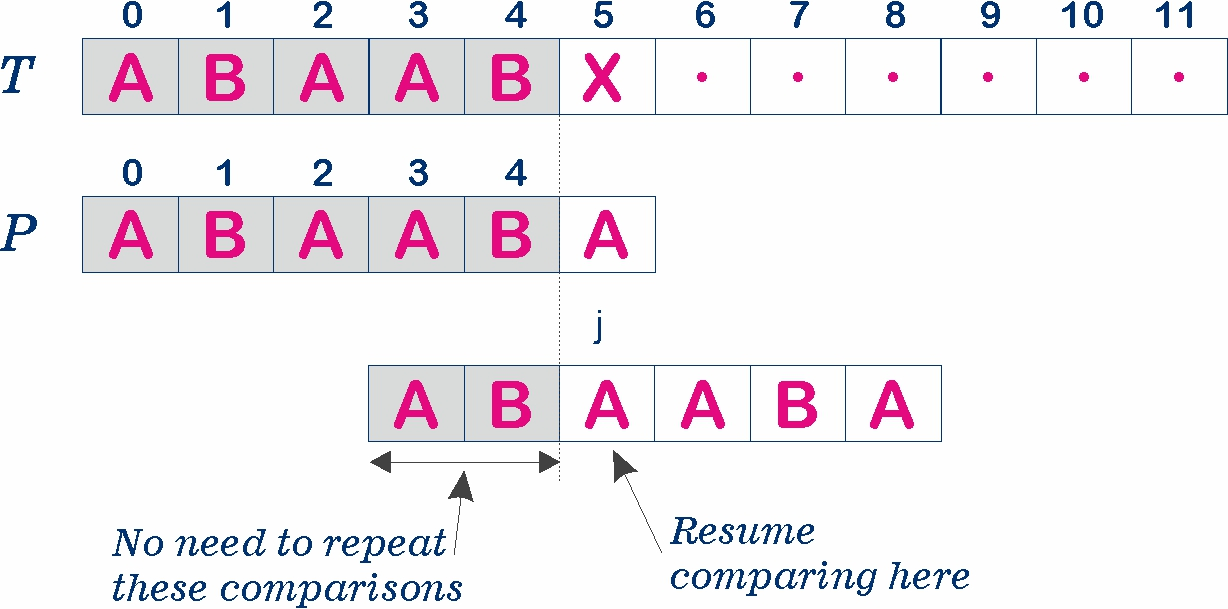
\includegraphics[width=12cm]{Images/kmp-mismatch.jpg}
\end{center}

\subsection{Tiền xử lý (xây dựng mảng LPS)}

Ý tưởng cốt lõi của thuật toán KMP là tiền xử lý xâu mẫu để xây dựng mảng \textit{LPS (Longest Prefix Suffix)}. Mảng này lưu độ dài của tiền tố dài nhất đồng thời cũng là hậu tố của từng đoạn con của xâu mẫu.

Việc xây dựng mảng LPS giúp thuật toán xác định vị trí dịch chuyển hợp lý khi xảy ra sai khác, từ đó tránh việc so sánh lại các ký tự đã biết.

\textbf{Thuật toán xây dựng LPS:}

\begin{itemize}
    \item Khởi tạo $lps[0] = 0$ vì một ký tự đơn không có tiền tố hoặc hậu tố thực sự.
    \item Sử dụng hai biến: $len$ (độ dài tiền tố - hậu tố hiện tại) và $i$ (duyệt pattern), với $len = 0$, $i = 1$.
    \item Trong khi $i < m$:
    \begin{itemize}
        \item Nếu $pattern[len] = pattern[i]$:
        \[
        lps[i] = len + 1,\quad len = len + 1,\quad i = i + 1
        \]
        \item Nếu không khớp và $len \neq 0$:
        \[
        len = lps[len - 1]
        \]
        \item Nếu không khớp và $len = 0$:
        \[
        lps[i] = 0,\quad i = i + 1
        \]
    \end{itemize}
\end{itemize}

\begin{center}
    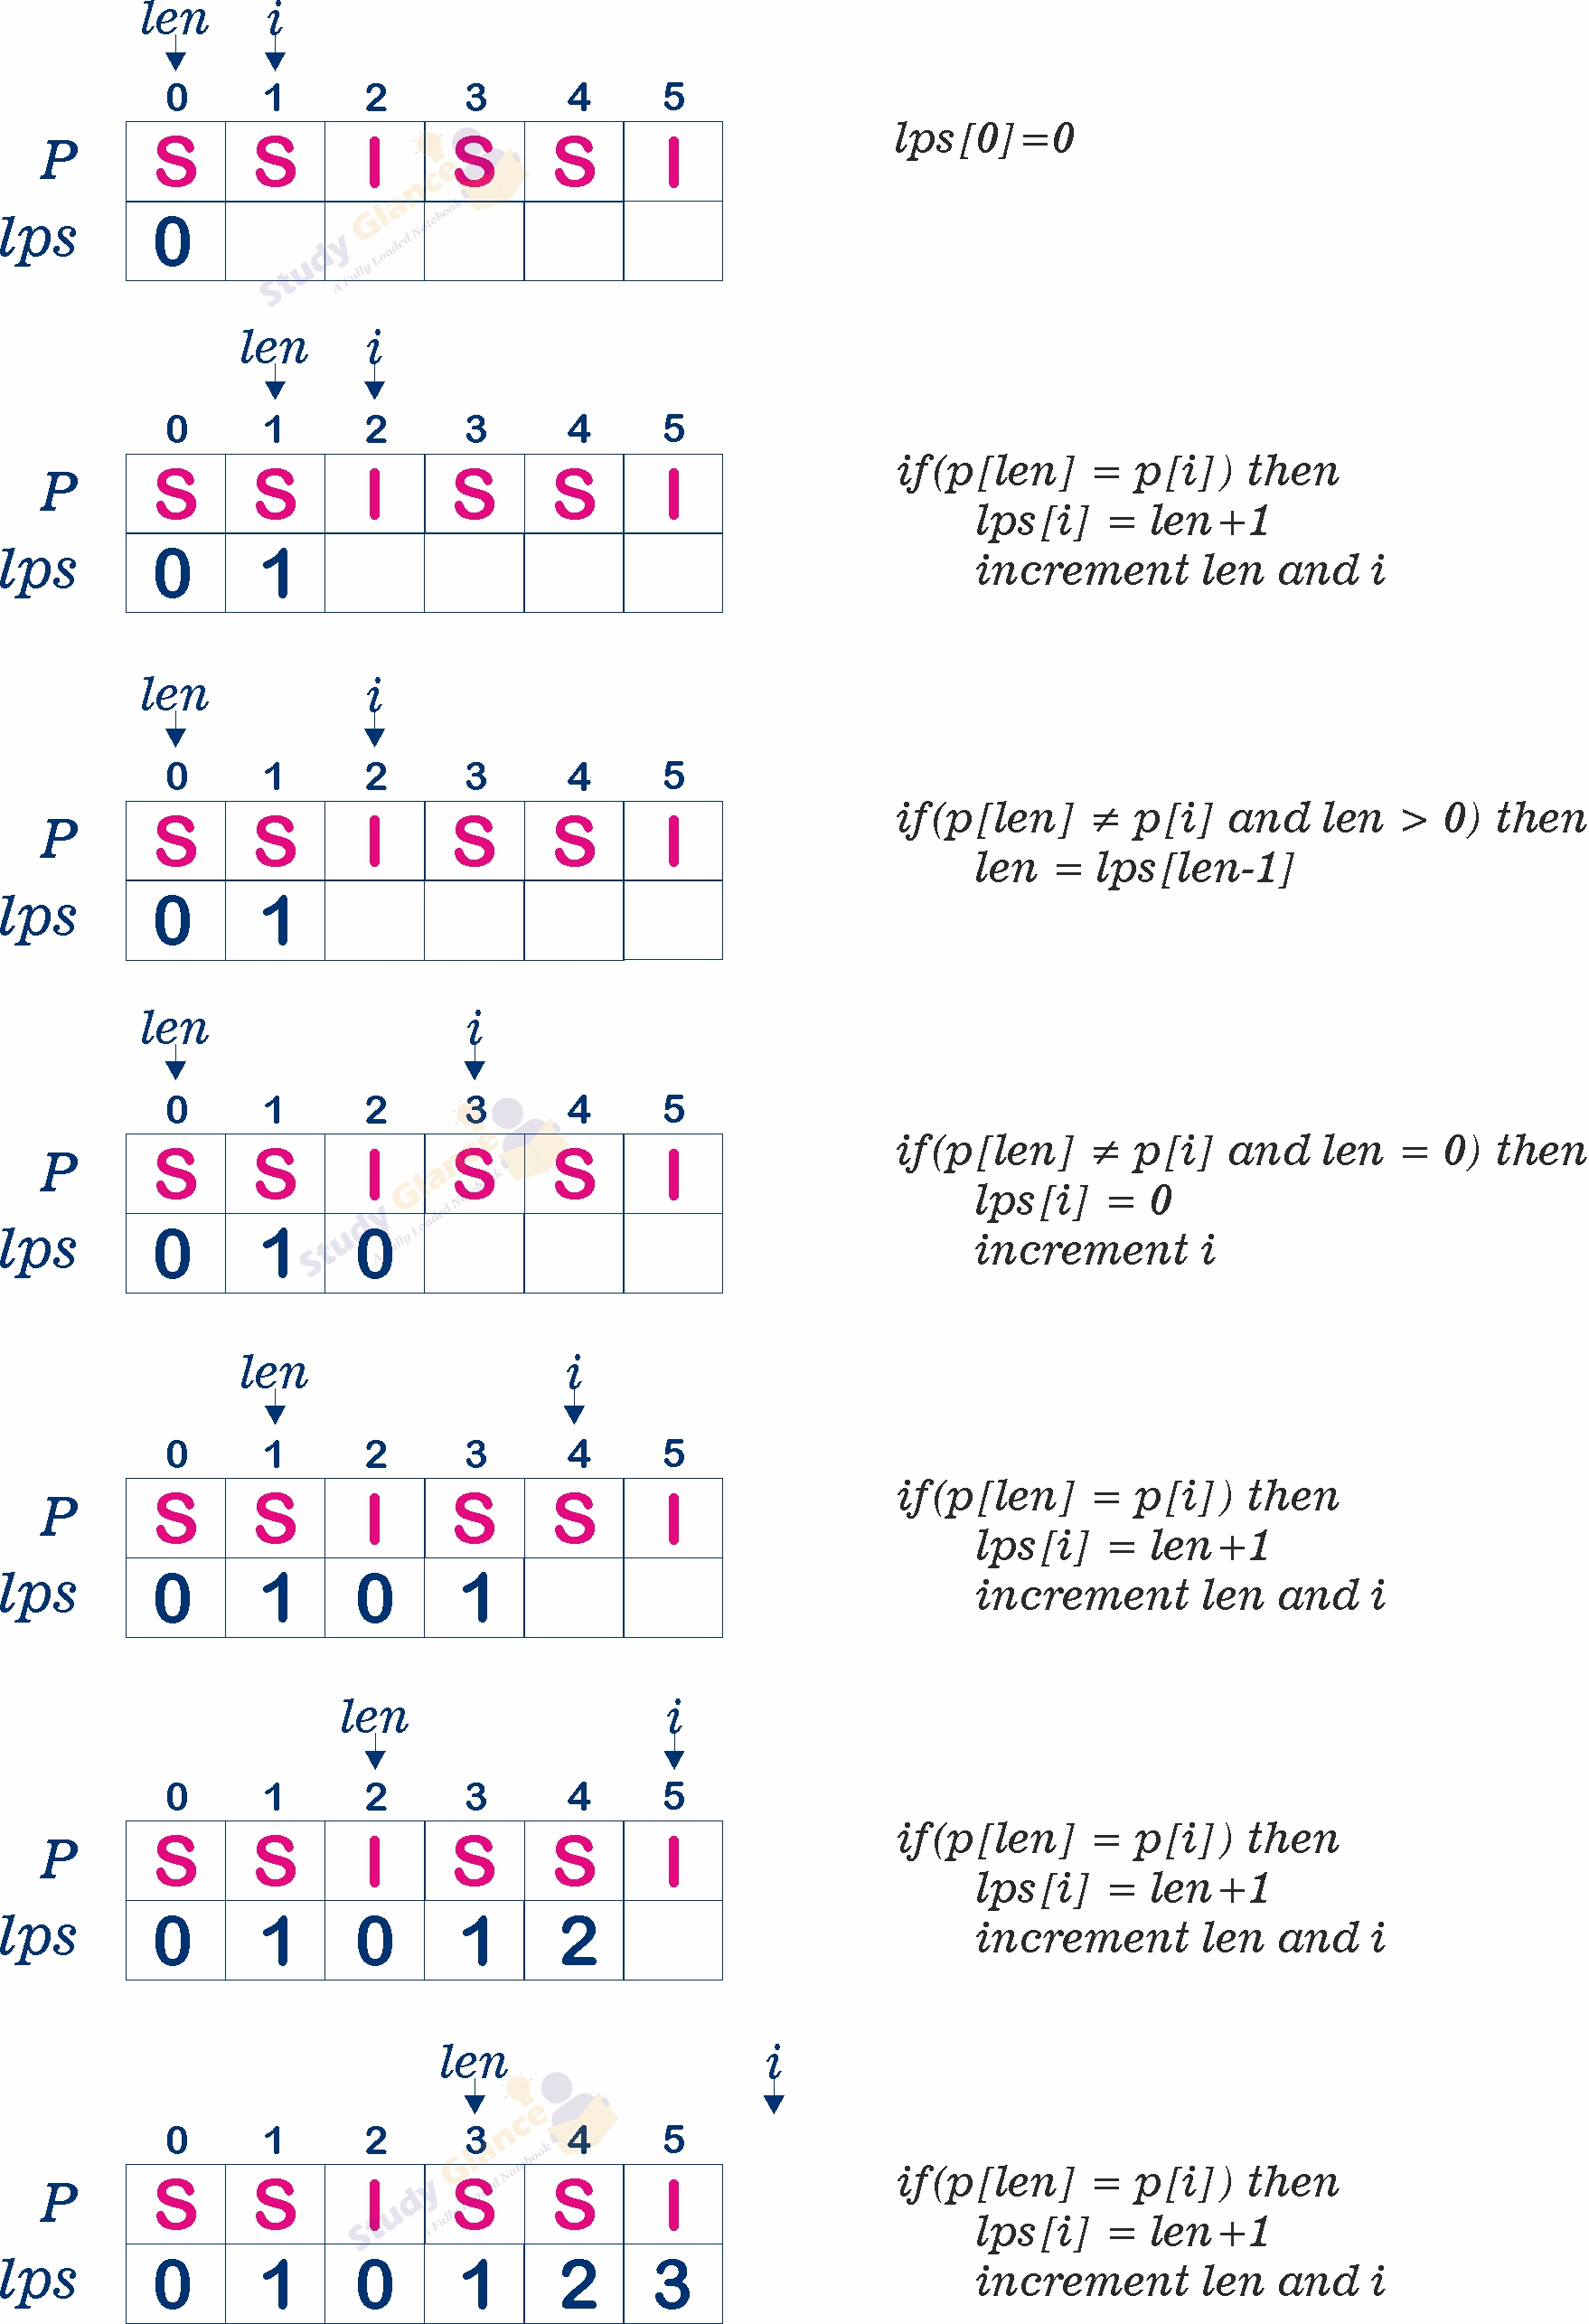
\includegraphics[width=12cm]{Images/Longest-Prefix-Suffix-lpstable.jpg}
\end{center}


\subsection{Quá trình tìm kiếm}

Sau khi hoàn tất bước tiền xử lý, thuật toán bắt đầu tìm kiếm trong văn bản.

\begin{itemize}
    \item Căn chỉnh xâu mẫu với đầu văn bản.
    \item So sánh ký tự của mẫu và văn bản từ trái sang phải.
    \item Nếu toàn bộ ký tự khớp, ghi nhận một lần xuất hiện của mẫu.
\end{itemize}

\subsection{Quá trình dịch chuyển}

Khi xảy ra sai khác tại vị trí $j$:

\begin{itemize}
    \item Nếu $pattern[j] = text[i]$, tăng cả $i$ và $j$.
    \item Nếu $j = m$, một lần khớp được tìm thấy, sau đó đặt $j = lps[j - 1]$.
    \item Nếu xảy ra sai khác và $j \neq 0$, cập nhật $j = lps[j - 1]$ (không tăng $i$).
    \item Nếu xảy ra sai khác và $j = 0$, tăng $i$.
\end{itemize}

\begin{center}
    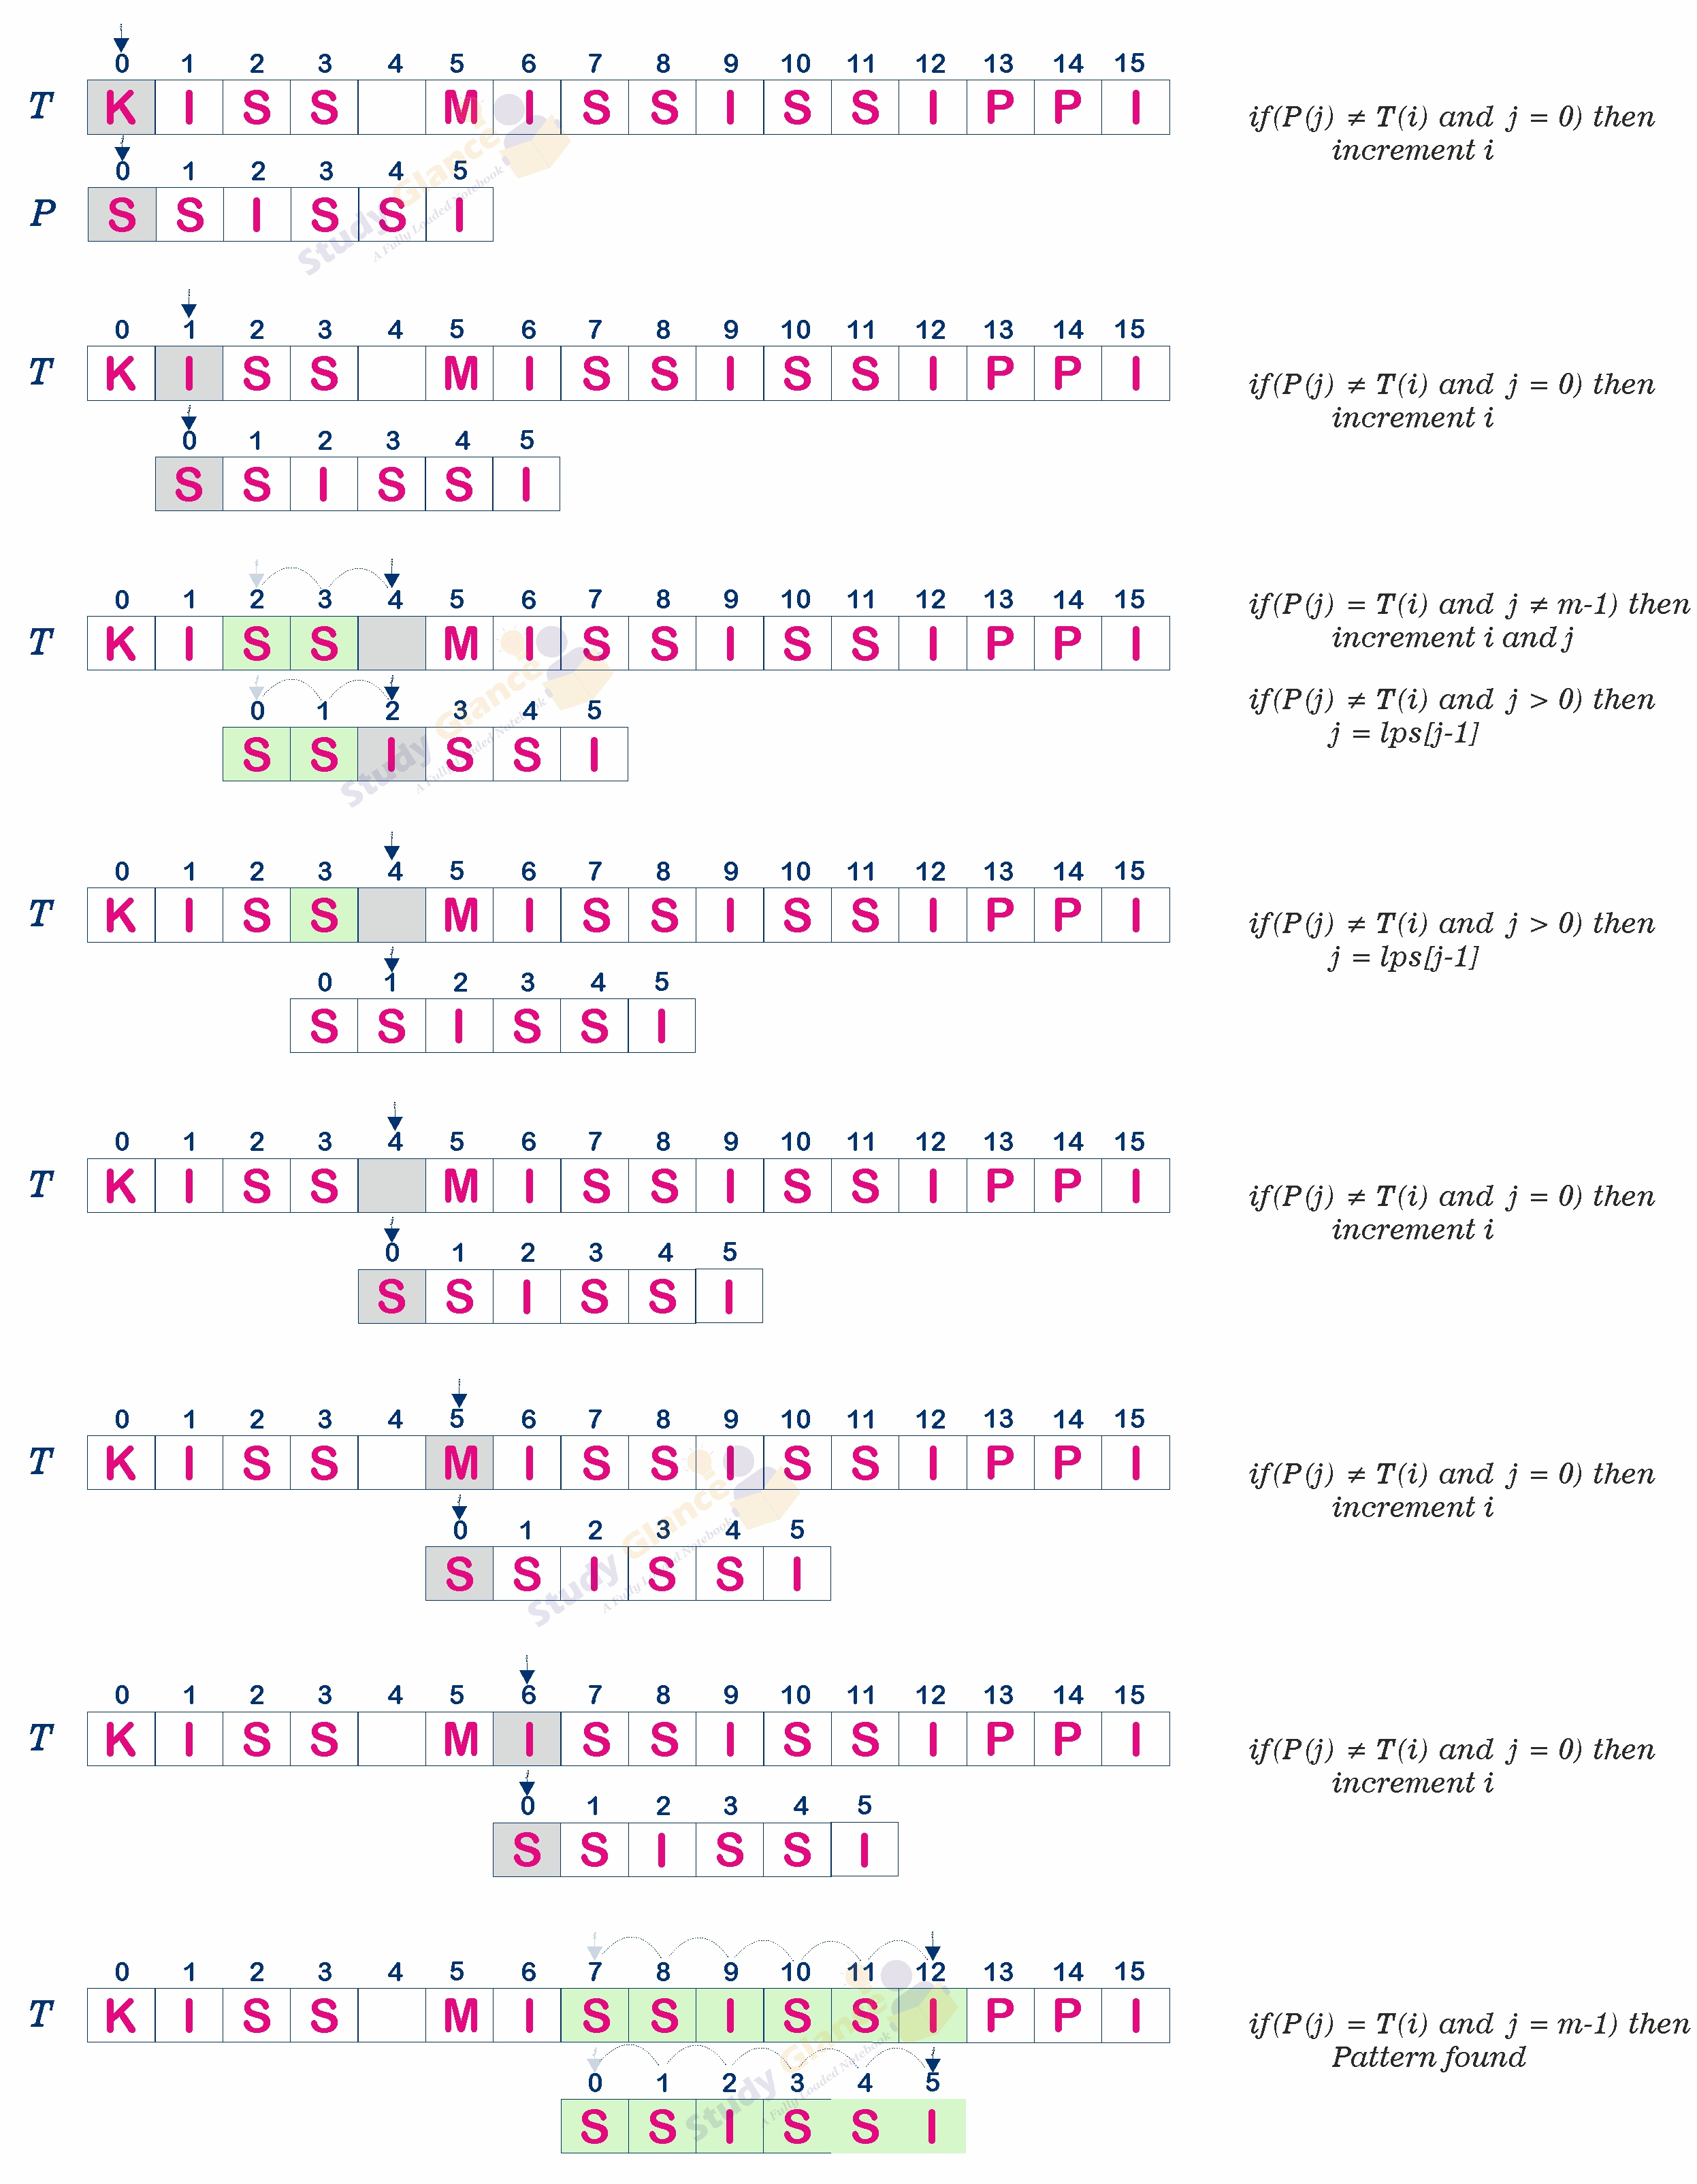
\includegraphics[width=12cm]{Images/kmp-Algorithm-in-data-structures.jpg}
\end{center}

\subsection{Lặp lại và kết thúc}

Thuật toán tiếp tục quá trình so sánh cho đến khi:

\begin{itemize}
    \item Duyệt hết văn bản, hoặc
    \item Tìm được tất cả các vị trí xuất hiện của mẫu trong văn bản.
\end{itemize}

\subsection{Cài đặt thuật toán bằng C++}

\begin{verbatim}
#include <iostream>
#include <vector>
#include <string>
using namespace std;

// Hàm xây dựng mảng LPS
vector<int> buildLPS(string pattern) {
    int m = pattern.size();
    vector<int> lps(m, 0);

    int len = 0; // độ dài prefix suffix
    int i = 1;

    while (i < m) {
        if (pattern[i] == pattern[len]) {
            len++;
            lps[i] = len;
            i++;
        }
        else {
            if (len != 0) {
                len = lps[len - 1];
            } else {
                lps[i] = 0;
                i++;
            }
        }
    }

    return lps;
}

// Hàm tìm kiếm KMP
vector<int> KMP(string text, string pattern) {
    vector<int> result;

    int n = text.size();
    int m = pattern.size();

    vector<int> lps = buildLPS(pattern);

    int i = 0; // index text
    int j = 0; // index pattern

    while (i < n) {
        if (text[i] == pattern[j]) {
            i++;
            j++;
        }

        if (j == m) {
            result.push_back(i - j);
            j = lps[j - 1];
        }
        else if (i < n && text[i] != pattern[j]) {
            if (j != 0)
                j = lps[j - 1];
            else
                i++;
        }
    }

    return result;
}

int main() {
    string text = "ababcabcabababd";
    string pattern = "ababd";

    vector<int> pos = KMP(text, pattern);

    cout << "Vi tri xuat hien: ";
    for (int x : pos) {
        cout << x << " ";
    }

    return 0;
}
\end{verbatim}